\documentclass[a3paper, border=20pt]{standalone}
\usepackage{tikz}
\usetikzlibrary{shapes, arrows, positioning}
\usetikzlibrary{fit}
\usetikzlibrary{matrix}
\usepackage{amsmath}

\begin{document}
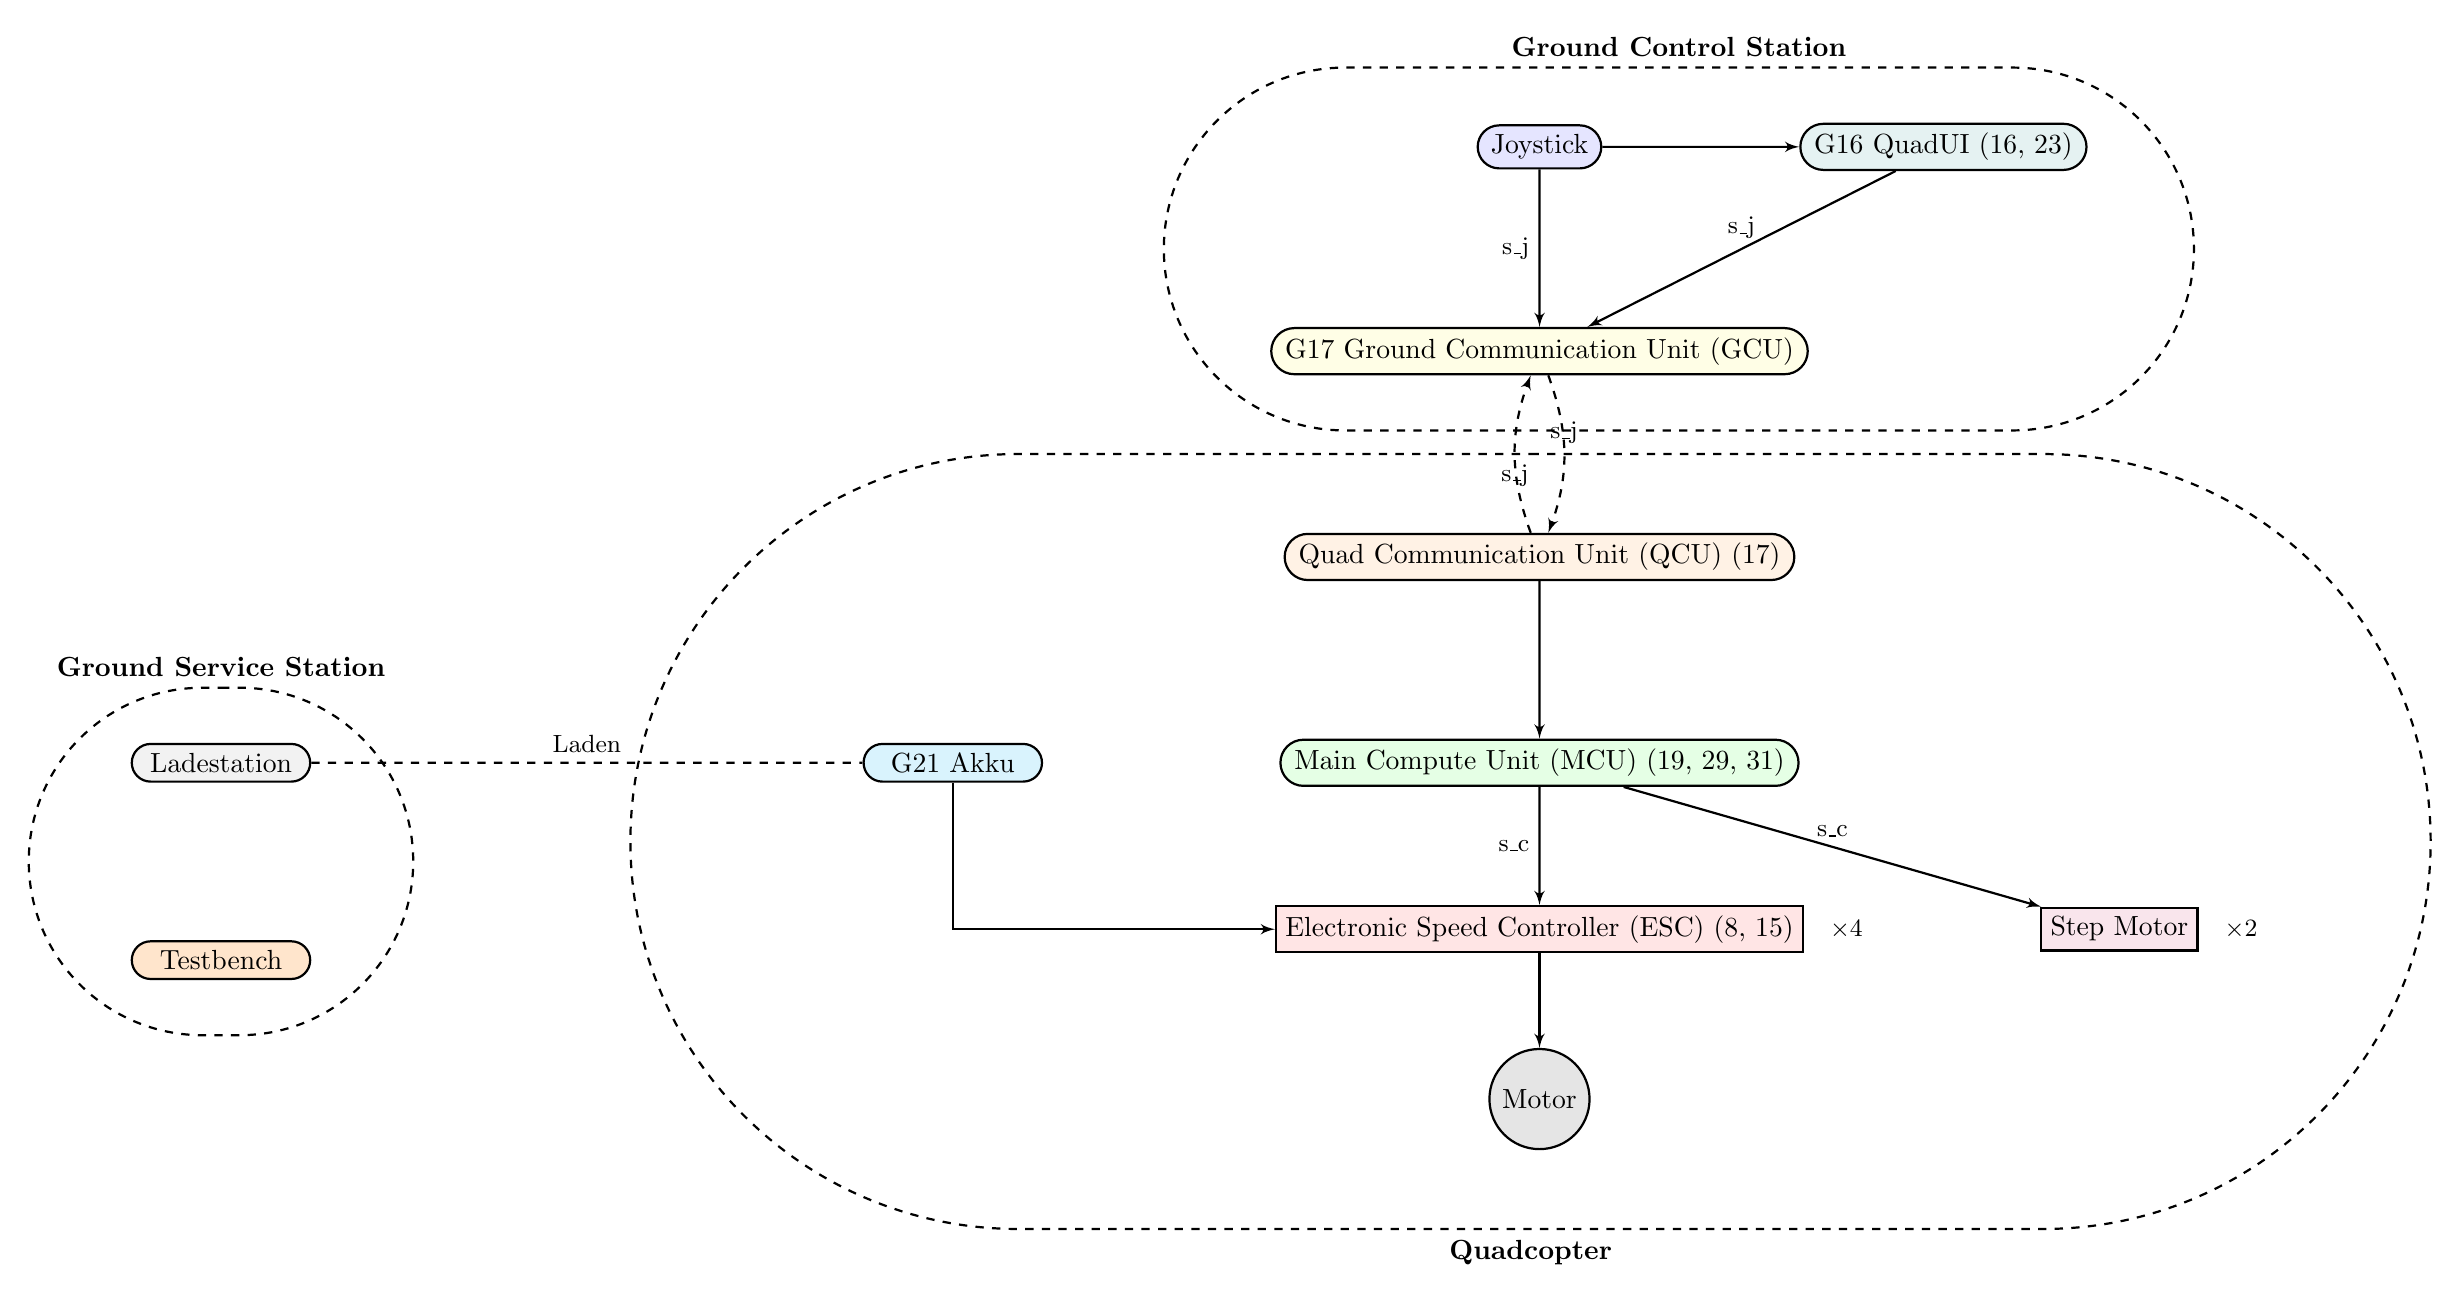
\begin{tikzpicture}[node distance=2cm, auto, >=latex', thick, xshift=2cm, yshift=2cm]
  % Vertikale Anordnung: Joystick, QuadUI, Communication Units, MCU
  \node[draw, rounded rectangle, fill=blue!10] (joystick) {Joystick};
  \node[draw, rounded rectangle, right=2.5cm of joystick, fill=teal!10] (quadui) {G16 QuadUI (16, 23)};
  \node[draw, rounded rectangle, below=2cm of joystick, fill=yellow!10] (gcu) {G17 Ground Communication Unit (GCU)};
  \node[draw, rounded rectangle, below=2cm of gcu, fill=orange!10] (rx) {Quad Communication Unit (QCU) (17)};
  \node[draw, rounded rectangle, below=2cm of rx, fill=green!10, minimum width=3cm] (mcu) {Main Compute Unit (MCU) (19, 29, 31)};
  % Akku, Ladestation und Testbench
  \node[draw, rounded rectangle, fill=cyan!15, left=3cm of mcu, minimum width=2.5cm] (akku) {G21 Akku};
  \node[draw, rounded rectangle, fill=gray!10, left=7cm of akku, minimum width=2.5cm] (ladestation) {Ladestation};
  \node[draw, rounded rectangle, fill=orange!20, below=2cm of ladestation, minimum width=2.5cm] (testbench) {Testbench};
  \draw[dashed, thick] (ladestation) -- node[above, font=\small]{Laden} (akku);

  % ESC and Motor (single representation for 4 units)
  \node[draw, rectangle, below=1.5cm of mcu, fill=red!10] (esc) {Electronic Speed Controller (ESC) (8, 15)};
  \node[draw, circle, below=1.2cm of esc, fill=gray!20] (motor) {Motor};
  \node[right=0.2cm of esc, font=\small\bfseries] {$\times 4$};
  \draw[->] (mcu) -- node[left, font=\small]{s\_c} (esc);
  \draw[->] (esc) -- (motor);
  \draw[->, thick] (akku) |- (esc);

  % Step Motor (single representation for 2 units)
  \node[draw, rectangle, right=3cm of esc, fill=purple!10] (step) {Step Motor};
  \node[right=0.2cm of step, font=\small\bfseries] {$\times 2$};
  \draw[->] (mcu) -- node[above, font=\small]{s\_c} (step);

  % Connections
  \draw[->] (joystick) -- (quadui);
  \draw[->] (joystick) -- node[left, font=\small]{s\_j} (gcu);
  \draw[->] (quadui) -- node[above, font=\small]{s\_j} (gcu);
  % Bidirektionale Kommunikation zwischen den Communication Units
  \draw[->, dashed, bend left=20] (gcu) to node[above, font=\small]{s\_j} (rx);
  \draw[->, dashed, bend left=20] (rx) to node[below, font=\small]{s\_j} (gcu);
  \draw[->] (rx) -- (mcu);

  % Quadcopter-Komponenten-Box
  \node[draw, dashed, rounded rectangle, fit=(mcu) (esc) (motor) (rx) (akku) (step), inner sep=1cm, label=below:{\textbf{Quadcopter}}] (quadbox) {};

  % Ground Control Station-Box
  \node[draw, dashed, rounded rectangle, fit=(joystick) (quadui) (gcu), inner sep=0.7cm, label=above:{\textbf{Ground Control Station}}] (gcsbox) {};

  % Ground Service Station-Box
  \node[draw, dashed, rounded rectangle, fit=(ladestation) (testbench), inner sep=0.7cm, label=above:{\textbf{Ground Service Station}}] (gssbox) {};
\end{tikzpicture}

% Legende
\vspace{1cm}
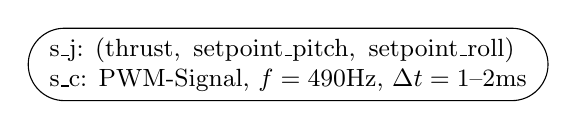
\begin{tikzpicture}
  \node[draw, fill=white!90, rounded rectangle, font=\small, align=left] at (0,0) {
    s\_j: $(\text{thrust},\ \text{setpoint\_pitch},\ \text{setpoint\_roll})$\\
    s\_c: PWM-Signal, $f=490$Hz, $\Delta t=1$--$2$ms
  };
\end{tikzpicture}
\end{document}